\documentclass{article}
\usepackage[utf8]{inputenc}

\usepackage{amsmath}
\usepackage{graphicx}
\usepackage{indentfirst}

%--------Margin of the page------------%
\usepackage[margin=1in]{geometry}

%--------Code Snipplet Setting------------%
\usepackage{listings}
\usepackage{xcolor}

\definecolor{codegreen}{rgb}{0,0.6,0}
\definecolor{codegray}{rgb}{0.5,0.5,0.5}
\definecolor{codepurple}{rgb}{0.58,0,0.82}
\definecolor{backcolour}{rgb}{0.95,0.95,0.92}

\lstdefinestyle{mystyle}{
    backgroundcolor=\color{backcolour},   
    commentstyle=\color{codegreen},
    keywordstyle=\color{magenta},
    numberstyle=\tiny\color{codegray},
    stringstyle=\color{codepurple},
    basicstyle=\ttfamily\footnotesize,
    breakatwhitespace=false,         
    breaklines=true,                 
    captionpos=b,                    
    keepspaces=true,                 
    numbers=left,                    
    numbersep=5pt,                  
    showspaces=false,                
    showstringspaces=false,
    showtabs=false,                  
    tabsize=2
}

\lstset{style=mystyle}
%--------Code Snipplet Setting------------%

\begin{document}

\section*{Newton's method to find a root of equations system.}

This example tries to find any one of the roots of below nonlinear system:
\begin{align*}
    x_1^2 + x_2^2 - 1 &= 0 \\
    5x_1^2 - x_2 - 2 &= 0
\end{align*}

This is the code for Newton-Raphson algorithm.

\lstinputlisting[language=Matlab]{newton.m}

This is the code for the particular function handling.

\lstinputlisting[language=Matlab]{FunctionName.m}

This is the main script file, together with the code used to generate the table result.

\lstinputlisting[language=Matlab]{script_test.m}

The result is reported as in this table.

\lstinputlisting[]{result.txt}

\begin{figure}[h]
    \centering
    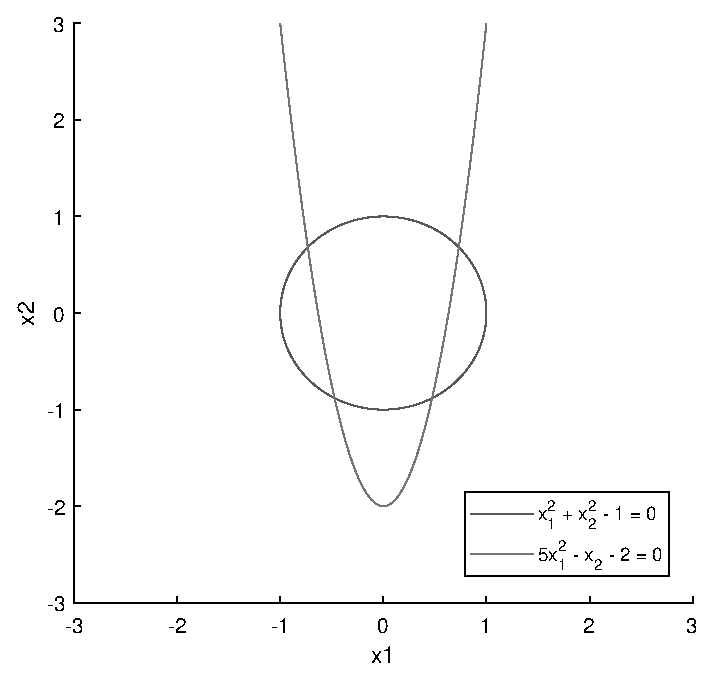
\includegraphics[width = 0.7\textwidth]{graph}
    \caption{The graphs of $x_1^2 + x_2^2 - 1 = 0$ and $5x_1^2 - x_2 - 2 = 0$.}
\end{figure}

From the graphic, there are 4 solutions in this nonlinear system. The result from the iteration, $(x_1,x_2) = (0.732,0.681)$ is represented by the upper-right point of the 4 intersection points (which are the solutions of nonlinear system.) 

\end{document}